% Chapter 2: Lit Review
\chapter{Literature Review}
\label{chapter:lit-review}

\graphicspath{ {report/C2 Literature Review/assets/} } 

% 2.1: EEG and neuroanatomy
\section{Electroencephalography (EEG) and Functional Neuroimaging}

\subsection{Basic electrophysiology}
EEG relies on electrophysiological activity generated by electro-chemical neurotransmitters that exchange signals between neurons in the brain \cite{bci-survey-nicolas-alonso}. Roughly speaking, when a neuron is excited by afferent action potentials (rapid changes in cell membrane potentials), postsynaptic potentials (EPSPs) are generated in its apical dendrites \cite{baillet-em-brain-mapping} (neural branches). This induces a potential difference (dipole) which results in a small flow of current from the nonexcited soma membrane to the apical dendrites where the EPSPs are present. \cite{baillet-em-brain-mapping}. This process causes both intracellular current flow within the neuron, as well as extracellular current flow. These current flows are termed \textit{primary} and \textit{secondary} or \textit{return} currents respectively. Both such currents contribute to electrical potentials measured on the scalp, however, it is believed that the source of most measurable EEG potentials arises from large collections of cortical pyramidal neurons arranged in macro-assemblies with dendrites orientated perpendicularly to the local cortical surface \cite{baillet-em-brain-mapping}, \cite{teplan-eeg-measurement}. The specific spatial positioning and simultaneous activation of these large clusters of neurons is believed to generate signals that can be measured on the scalp. Specifically, \cite{baillet-em-brain-mapping} suggests that these signals most likely arise from EPSPs in these macro-assemblies and less so due to rapidly firing action potentials that travel along the axons of excited neurons.

\subsection{Functional neuroimaging}
Various techniques exist for measuring and translating brain activity into electrical signals. These techniques are typically grouped into electrophysiological and hemodynamic. Hemodynamic techniques such as functional magnetic resonance (fMRI) and near infrared (NIR) spectroscopy measure brain activity \textit{indirectly }by tracking relative concentrations of oxyhemoglobin. The blood releases glucose to \textit{active} neurons at a greater rate than inactive ones which causes an increase in oxyhemoglobin in these active areas \cite{bci-survey-nicolas-alonso}, thereby providing a measurable proxy for cerebral activity. While hemodynamic approaches offer superior spatial resolution, they typically offer far lower temporal resolution and require complex, expensive equipment. 

EEG, on the other hand, is a electrophysiological technique that relies on the direct measurement of electrical signals generated by neural cell assemblies. Owing to the fact that it offers high temporal resolution\footnote{typically in the order of tens of milliseconds}, far lower cost than most other techniques, high portability and safety, EEG has become the most widely used neuroimaging modality \cite{bci-survey-nicolas-alonso}. It is these factors that make EEG the most appropriate modality for this project.

\subsection{Electroencephalography}

\subsubsection{Invasive vs non-invasive techniques}

The ability to reliably detect EEG signals is made challenging by the fact that neuron potentials must pass through the skull and scalp and will unavoidably be measured in conjunction with background noise and other undesirable artefacts such as electromyography (EMG) signals. Invasive methods that require surgical implantation of electronic devices are sometimes used in order to circumvent some of these challenges. Electrocorticography or intercranial EEG is an example of an invasive method; an electrode array is placed directly on the exposed surface of the brain to measure cerebral activity. 

While invasive methods offer superior signal resolution and quality, they are clearly not suitable for this project. Non-invasive BCIs do not require any surgical intervention and only involve the placement of electrodes on the scalp of the subject. Despite the aforementioned challenges of measuring signals of poorer quality, this has the advantage of convenience, cost effectiveness, safety and minimal invasiveness.

\subsubsection{The nature of EEG signals}
EEG signals, or 'brain waves', commonly follow a roughly sinusoidal shape in nature and range in amplitude from 0.5 to $100\mu$V peak-to-peak \cite{teplan-eeg-measurement} (in the case of a healthy brain). For reference, this is roughly 100 times lower than the typical amplitude of ECG signals. It is widely believed that EEG signals show varying energy in a few distinct frequency bands depending on mental state and cognitive function of a subject \cite{baillet-em-brain-mapping}, \cite{varnavas-phd}. These frequency bands are summarised below \cite{varnavas-phd}, \cite{bci-survey-nicolas-alonso}:

\begin{table}[!htb]
\centering
\begin{tabular}{@{}ll@{}}
\toprule
\textbf{Frequency Band} &
  \textbf{Association} \\ \midrule
delta (0.5 - 4Hz) &
  \begin{tabular}[c]{@{}l@{}}Usually only detected in a state of deep sleep. Excessive signal energy in the delta band \\ while awake may suggest neurological disease.\end{tabular} \\
theta (4 - 8Hz) &
  \begin{tabular}[c]{@{}l@{}}Cognitive tasks involving association, awareness and meditation. Usually low energy\\ in this band while subject is awake.\end{tabular} \\
alpha (8 - 13Hz) &
  \begin{tabular}[c]{@{}l@{}}Typically measured in the occipital region of the brain. Primarily related to visual processing \\ but also memory processes. Induced by closing of the eyes and relaxing and attenuated when \\ eyes are open or by thinking or mental calculation.\end{tabular} \\
beta (12 - 30Hz) &
  \begin{tabular}[c]{@{}l@{}}A variety of mental processes such as mathematical computation, planning, high \\ level processing\end{tabular} \\ \bottomrule
\end{tabular}
\caption{MPSE of ANC vs ALE averaged across 100 realisations}
\label{tab:c2-freq-bands}
\end{table}

It is worth noting that different areas of the brain may produce signals with different energy compositions across these frequency bands. Consequently, the particular placement of electrodes in measuring localised signals of interest is an important consideration.

\subsubsection{Electrode choice and placement}
An EEG is signal is most commonly measured as the potential difference over time between active and reference electrodes. A third ground electrode is used to measure differential voltage between the active and reference electrodes and thus, a minimal setup requires at least 3 electrodes in total \cite{bci-survey-nicolas-alonso}. Electrodes be used in conjunction with conductive media such as conductive gel or without and would be termed wet or dry electrodes in these two cases respectively. 

Electrodes are most commonly arranged on the scalp according to the International 10-20 system standardised by the American Electroencephalographic Society. An overview of this system is presented in Figure \ref{fig:10-20-positions}.

\begin{figure}[h]
    \centering
    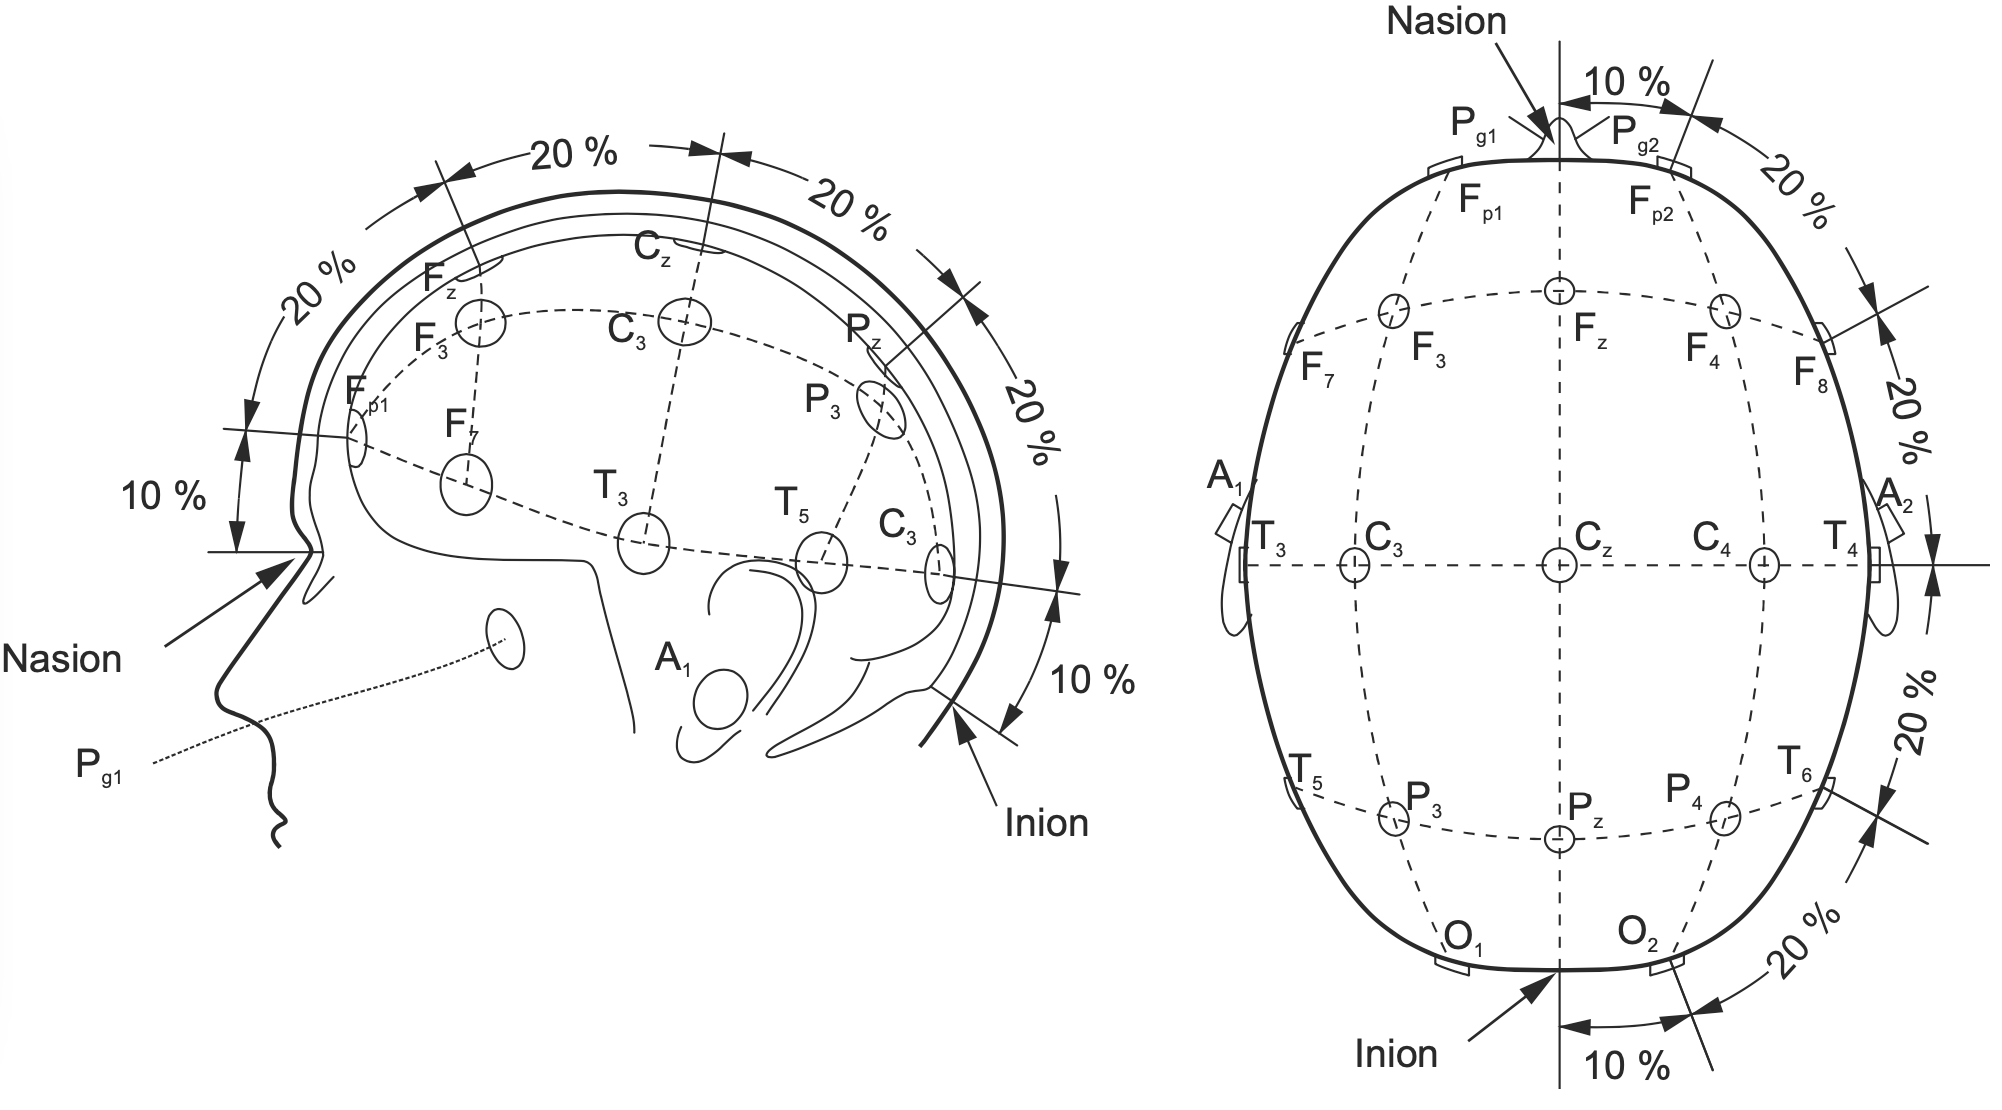
\includegraphics[width=0.8\textwidth]{10-20-electrode.png}
    \caption[Electrode positions according to the 10-20 system]{Diagram illustrating typical electrode placements using the international 10-20 system. A represents the ear lobe, C the central region, P the parietal, F the frontal and O the occipital. The \textit{naison} and \textit{inion} are used as reference locations.}
    \label{fig:10-20-positions}
\end{figure}

\subsection{EEG Paradigms}
As alluded to before, one of the objectives for the Royal Society Exhibition is to create a multiplayer game that receives control signals from participants in the audience wearing our EEG devices. Thus, one of the responsibilities of this project is to decide on the specific EEG paradigm that will be used to capture user input. It should be noted that the feasibility of various paradigms largely depends on the quality of the available signals and that of the decoding pipeline which are yet to be conclusively determined. Several studies suggest that \textbf{steady-state visual evoked potentials} \cite{Fernandez-Fraga2016}\cite{Kanoga2020}\cite{Acampora2021} (SSVEPs) offer significant potential for EEG decoding tasks similar to this project due to the high information transfer rate (ITR), non-invasiveness and relatively high SNR that can be achieved using basic BCI devices \cite{Zhu2021}. 

\subsection{Steady-state visual evoked potentials (SSVEP)}
An SSVEP signal is most commonly observed as the brain's response to a visual stimulus flickering at constant frequency \cite{Xie2016}. Specifically, the fundamental SSVEP frequency $f_{SSVEP}^{(0)}$ will match that of the stimulus in the spectrum of the resulting EEG signal (within some frequency bounds, as explored below). Stimulus frequency bands of around 8-15Hz are commonly used \cite{Acampora2021}\cite{Chen2017}, however, Xie et al showed successful decoding with 27.8Hz \cite{Xie2016}. SSVEPs are produced in the brain's visual cortex and are usually measured in the occipital and/or parietal regions \cite{Fernandez-Fraga2016}. Using the international 10-20 electrode electrode scheme, this corresponds to the $\text{PO}_x$ and $\text{O}_x$  electrodes. The current idea is that users in the exhibition will be presented a mobile-friendly, lightweight web page with 2-4 stimulus squares or other images that flicker at frequencies $f_1, \dots, f_n$. Each stimulus will correspond to an action - such as `up' or `down' - that will control an avatar in the cooperative game mentioned above. The objective is to decode $f_1, \dots, f_n$ in order to interpret a user's desired action (i.e. discern which stimulus image they are focused on).

% 2.2: EEG Mechanics
\section{EEG Signal Acquisition and Processing}
Discuss the state-of-the-art in EEG signal acquisition and processing techniques. Discuss the mechanics of existing, commonly used devices both in industry and academia.
\subsection{Experimental parameters in SSVEP decoding and their implications}
\subsubsection{Number of EEG channels used}
\subsubsection{Characterisation of visual stimuli}
Discussion on parameters that can be changed in SSVEP experiments and the implications thereof:
\begin{itemize}
    \item Number of visual stimuli
    \item Contrast and colour
    \item Relative size and positioning of stimuli
    \item Frequencies
\end{itemize}

\subsection{Practical considerations}
Potentially list any practical findings from the literature that would influence our design choices. For example, refresh rate of screens and the impact on consistency of flickering stimuli. Or perhaps just the hardware that was used in experiments in the literature and the importance of that (if any)

\section{Computational Approaches for SSVEP Decoding}
\subsection{Power spectral density and frequency domain}
\subsection{Statistical}
\subsection{Data-driven and machine learning}